\documentclass[10pt,a4paper]{article}

% =========================
% Page + Font
% =========================
\usepackage[a4paper,left=1.6cm,right=1.6cm,top=1.4cm,bottom=1.4cm]{geometry}
\usepackage[T1]{fontenc}
\usepackage[utf8]{inputenc}
\usepackage{helvet}
\renewcommand{\familydefault}{\sfdefault}
\usepackage{microtype}
\usepackage{setspace}

% =========================
% Tables + Colors + Figures
% =========================
\usepackage[table]{xcolor}
\usepackage{colortbl}
\usepackage{array}
\usepackage{tabularx}
\usepackage{booktabs}
\usepackage{makecell}
\usepackage{graphicx}
\usepackage{float}
\usepackage{caption}
\usepackage{ragged2e}
\usepackage{enumitem}

% =========================
% General formatting
% =========================
\pagestyle{empty}
\setlength{\parindent}{0pt}
\setlength{\parskip}{0.35em}
\setlength{\tabcolsep}{5pt}
\renewcommand{\arraystretch}{1.17}
\captionsetup{font=footnotesize}

% =========================
% Palette
% =========================
\definecolor{ReportBlue}{HTML}{0D2C54}
\definecolor{LightBlue}{HTML}{1E5799}
\definecolor{LightGray}{HTML}{F4F6F9}
\definecolor{MidGray}{HTML}{C8CDD6}
\definecolor{GoodGreen}{HTML}{1E7D46}
\definecolor{MetricRed}{HTML}{C0392B}
\definecolor{CaptionGray}{HTML}{666666}
\definecolor{BodyGray}{HTML}{333333}
\definecolor{FooterGray}{HTML}{999999}
\definecolor{KPIBlueBG}{HTML}{EAF0FB}
\definecolor{KPIGreenBG}{HTML}{E8F5EE}

% =========================
% Reusable macros
% =========================
\newcommand{\SectionBar}[1]{%
  \vspace{0.35em}
  \noindent\colorbox{ReportBlue}{%
    \parbox{\dimexpr\linewidth-2\fboxsep\relax}{%
      \vspace{2.5pt}\textcolor{white}{\bfseries\footnotesize #1}\vspace{2.5pt}
    }%
  }%
  \vspace{0.35em}
}

\begin{document}
\color{BodyGray}

% =========================
% Cover
% =========================
\begin{center}
  {\fontsize{17}{20}\selectfont\textbf{\textcolor{ReportBlue}{Portfolio Optimization Report - Assignment III}}}\par
  \vspace{3pt}
  {\fontsize{9}{11}\selectfont\textcolor{CaptionGray}{DA6701 - Data Science and AI in Finance}}\par
  \vspace{1pt}
  {\fontsize{9}{11}\selectfont\textcolor{CaptionGray}{Part I: Covariance Estimation and Ledoit-Wolf Shrinkage \quad | \quad Part II: Hierarchical Risk Parity (HRP)}}
\end{center}
\vspace{6pt}
\noindent\textcolor{ReportBlue}{\rule{\linewidth}{2pt}}

\vspace{8pt}
\SectionBar{1 \;|\; Objective, Universe, and Experimental Setup}
{\fontsize{8.1}{10.7}\selectfont\justifying
This report evaluates two portfolio construction frameworks on a 12-stock NSE universe: (i) covariance estimation and regularization effects in a maximum-Sharpe setting, and (ii) Hierarchical Risk Parity (HRP) using correlation-distance clustering and recursive risk allocation. The data window spans \textbf{January 2020 to December 2024} for Part I (monthly returns) and \textbf{January 2020 to December 2024} for Part II (daily returns). For HRP, the train/test split is \textbf{2020-01-02 to 2023-12-29} (train, 991 days) and \textbf{2024-01-01 to 2024-12-31} (test, 246 days).}

\SectionBar{2 \;|\; Part I (LW): Covariance Stability and Out-of-Sample Behavior}
{\fontsize{8.1}{10.7}\selectfont\justifying
The Part I notebook compares sample covariance and Ledoit-Wolf (LW) shrinkage in a maximum-Sharpe construction. The numerical diagnostics show clear conditioning gains under shrinkage:
\begin{itemize}[leftmargin=1.2em,itemsep=0.15em,topsep=0.2em]
  \item Returns covariance condition number: \textbf{97.87}
  \item Ledoit-Wolf covariance condition number: \textbf{26.33}
  \item Shrinkage intensity: \textbf{0.1661}
  \item Conditioning improvement factor: \textbf{3.7x}
\end{itemize}
Matrix-level differences remain meaningful but controlled (mean absolute difference \(= 0.0394\), max absolute difference \(= 0.1895\), Frobenius norm reduction \(0.83 \rightarrow 0.71\), relative change \(= 16.7\%\)).
}

{\fontsize{7.9}{10.4}\selectfont
\arrayrulecolor{MidGray}
\rowcolors{2}{LightGray}{white}
\begin{tabularx}{\linewidth}{|>{\RaggedRight\arraybackslash}X|>{\centering\arraybackslash}p{2.6cm}|>{\centering\arraybackslash}p{2.6cm}|}
  \hline
  \rowcolor{ReportBlue}
  \textcolor{white}{\textbf{Part I Out-of-Sample KPI}} &
  \textcolor{white}{\textbf{Returns Cov}} &
  \textcolor{white}{\textbf{Ledoit-Wolf Cov}} \\
  \hline
  Annual Return & 13.00\% & \textbf{16.03\%} \\
  Sharpe Ratio  & 2.737   & \textbf{5.333} \\
  \hline
\end{tabularx}
}

{\fontsize{7.6}{9.8}\selectfont\textcolor{CaptionGray}{
Note: The notebook print label mentions ``Out-of-Sample Performance (2025)'', while the displayed split indicates test months in 2024; this appears to be a labeling artifact rather than a data inconsistency.}}

\vspace{4pt}
\noindent
\begin{minipage}[t]{0.58\linewidth}
  \centering
  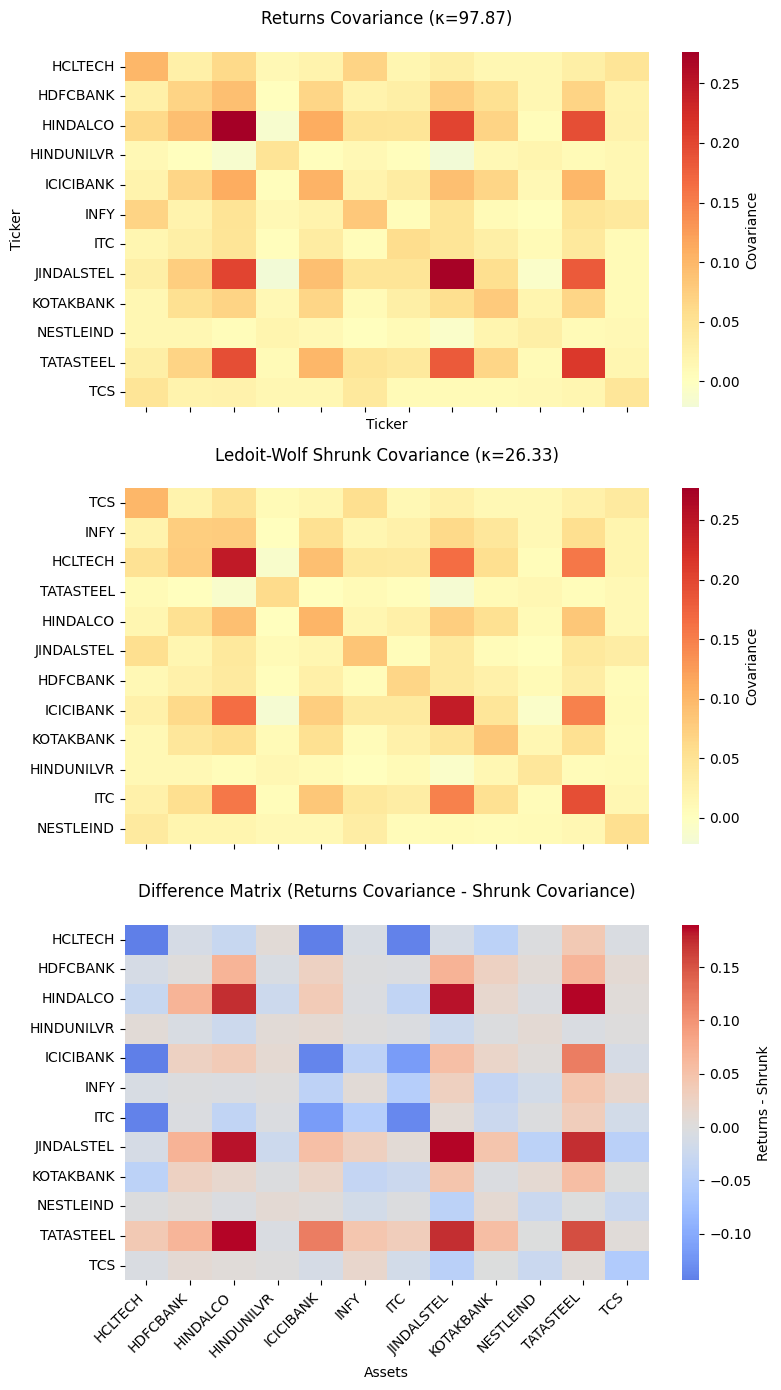
\includegraphics[width=\linewidth,height=7.0cm,keepaspectratio]{Visualization_1.png}
  \captionof{figure}{Part I (Compulsory Figure): Sample covariance, LW shrunk covariance, and their difference matrix.}
\end{minipage}
\hfill
\begin{minipage}[t]{0.40\linewidth}
  \centering
  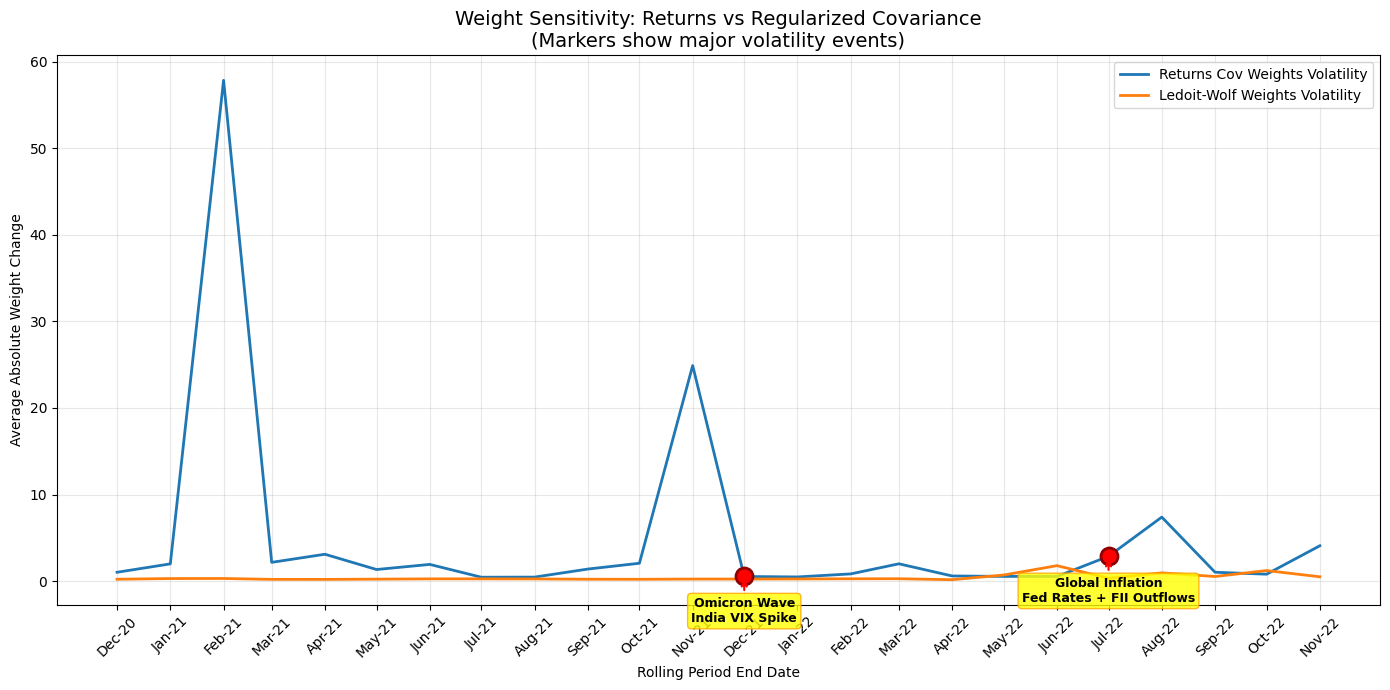
\includegraphics[width=\linewidth,height=7.0cm,keepaspectratio]{Visualization_3.png}
  \captionof{figure}{Part I (Compulsory Figure): Weight sensitivity over rolling periods.}
\end{minipage}

{\fontsize{8.0}{10.5}\selectfont\justifying
\textbf{Interpretation:} Visualization 1 confirms that shrinkage moderates noisy off-diagonal structure while preserving broad covariance blocks. Visualization 3 shows that sample-covariance-derived allocations are highly unstable during stress windows (notable spikes around Feb-2021 and Nov-2021), whereas LW-driven allocation updates remain materially smoother. Together, this supports LW as the more robust estimator for practical, repeated re-allocation workflows.
}

\SectionBar{3 \;|\; Part II (HRP): Clustering, Allocation, and Benchmark Comparison}
{\fontsize{8.1}{10.7}\selectfont\justifying
HRP uses the correlation-distance transformation \(D_{ij}=\sqrt{0.5(1-\rho_{ij})}\), single-linkage hierarchical clustering, quasi-diagonalization of covariance, and recursive bisection allocation. At distance cut \textbf{0.50}, the five economically interpretable clusters are:
}

{\fontsize{7.9}{10.3}\selectfont
\arrayrulecolor{MidGray}
\rowcolors{2}{LightGray}{white}
\begin{tabularx}{\linewidth}{|>{\centering\arraybackslash}p{1.5cm}|>{\RaggedRight\arraybackslash}X|>{\centering\arraybackslash}p{2.5cm}|>{\centering\arraybackslash}p{2.5cm}|}
  \hline
  \rowcolor{ReportBlue}
  \textcolor{white}{\textbf{Cluster}} &
  \textcolor{white}{\textbf{Members}} &
  \textcolor{white}{\textbf{Avg Intra-\(\rho\)}} &
  \textcolor{white}{\textbf{Volatility Range}} \\
  \hline
  1 & HINDUNILVR, NESTLEIND & 0.608 & 23.2\%--24.7\% \\
  2 & HCLTECH, INFY, TCS & 0.683 & 25.2\%--29.0\% \\
  3 & HINDALCO, JINDALSTEL, TATASTEEL & 0.745 & 39.3\%--50.0\% \\
  4 & HDFCBANK, ICICIBANK, KOTAKBANK & 0.641 & 28.4\%--33.9\% \\
  5 & ITC & 1.000 & 27.3\% \\
  \hline
\end{tabularx}
}

\begin{center}
  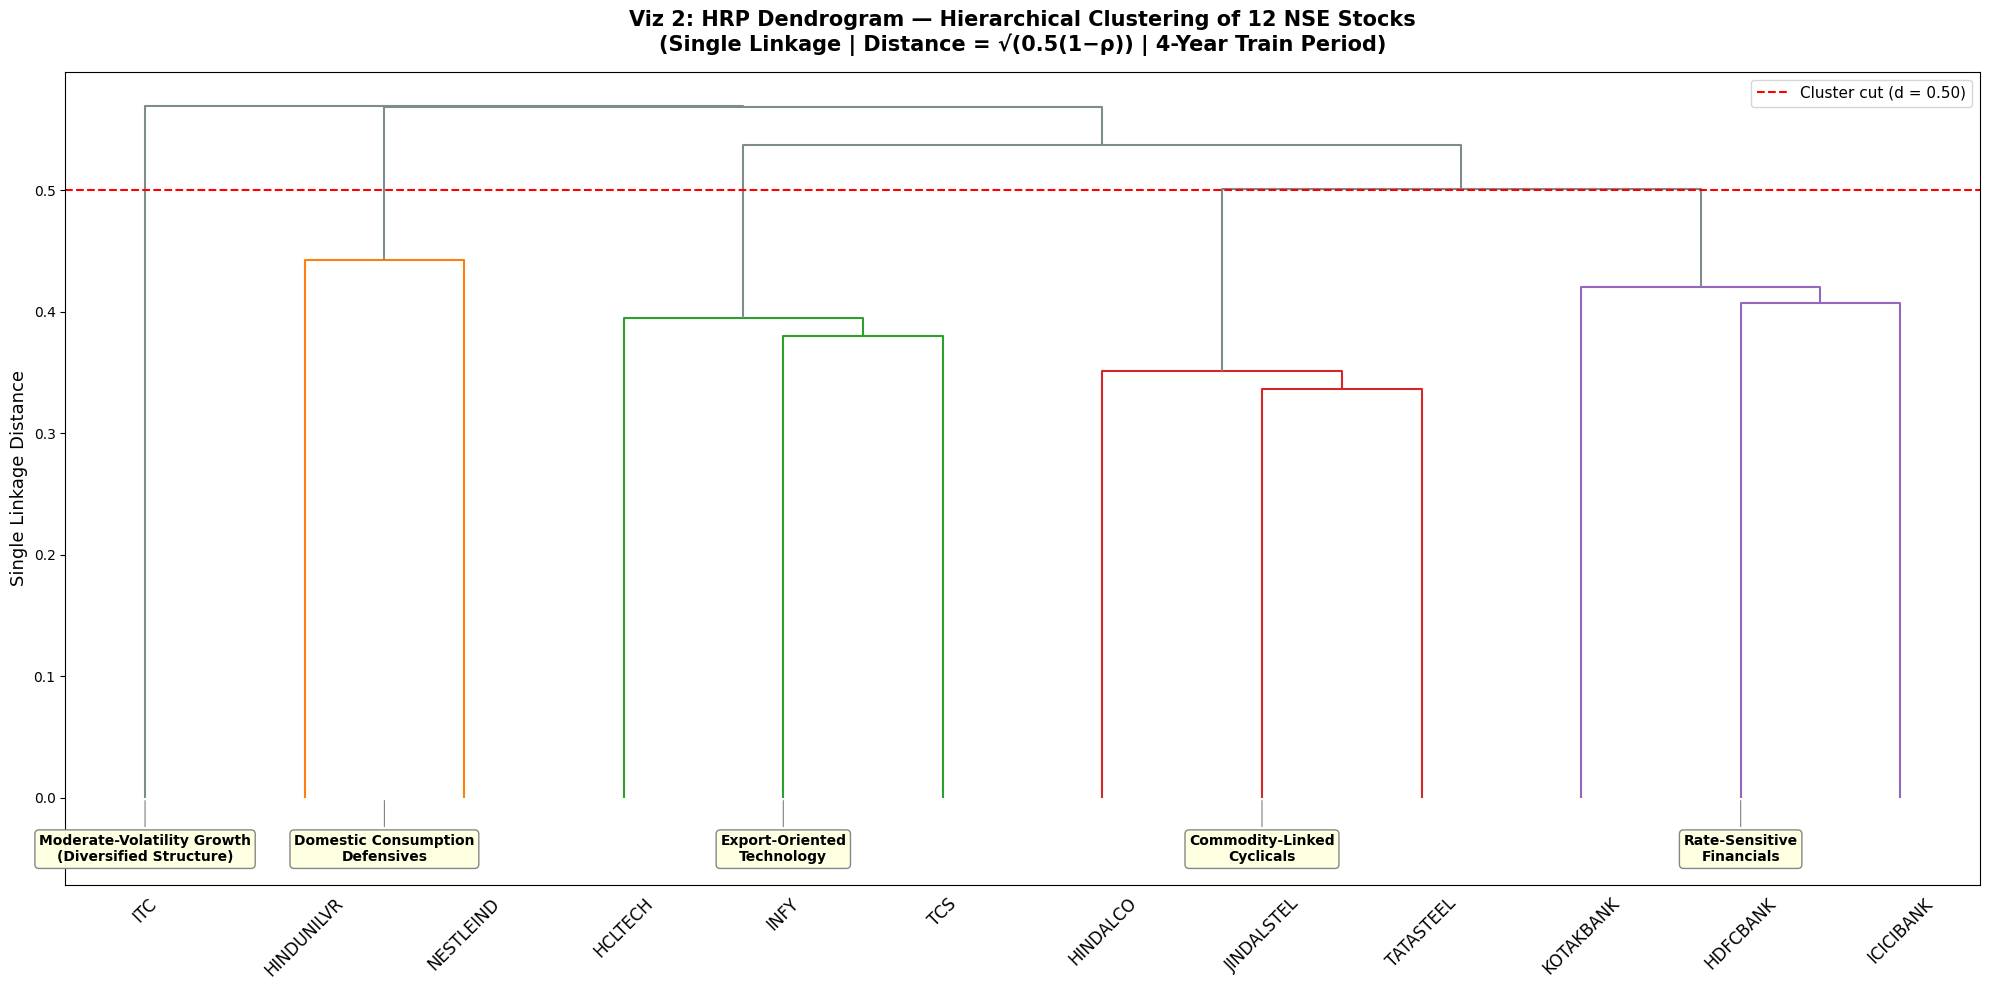
\includegraphics[width=\linewidth,height=7.8cm,keepaspectratio]{Visualization_2.png}
  \captionof{figure}{Part II (Compulsory Figure): HRP dendrogram with distance cut \(d=0.50\).}
\end{center}

{\fontsize{8.0}{10.5}\selectfont\justifying
\textbf{HRP Weights (descending):} ITC (16.32\%), NESTLEIND (14.12\%), HINDUNILVR (12.43\%), HCLTECH (11.02\%), KOTAKBANK (9.72\%), TCS (8.50\%), HDFCBANK (6.87\%), INFY (6.45\%), ICICIBANK (4.80\%), HINDALCO (4.60\%), TATASTEEL (3.20\%), JINDALSTEL (1.98\%).\\
\textbf{MPT In-sample (train) reference:} Annualized return \(=32.21\%\), annualized volatility \(=22.73\%\), Sharpe \(=1.1310\), with concentrated exposures (notably HCLTECH, ITC, JINDALSTEL, NESTLEIND, TATASTEEL).
}

{\fontsize{7.9}{10.3}\selectfont
\arrayrulecolor{MidGray}
\rowcolors{2}{LightGray}{white}
\begin{tabularx}{\linewidth}{|>{\RaggedRight\arraybackslash}X|>{\centering\arraybackslash}p{2.2cm}|>{\centering\arraybackslash}p{2.2cm}|}
  \hline
  \rowcolor{ReportBlue}
  \textcolor{white}{\textbf{2024 Test-Set Metric}} &
  \textcolor{white}{\textbf{HRP}} &
  \textcolor{white}{\textbf{MPT}} \\
  \hline
  Cumulative Return & 5.97\% & \textbf{17.30\%} \\
  Annualized Return & 6.12\% & \textbf{17.75\%} \\
  Annualized Volatility & \textbf{12.13\%} & 15.03\% \\
  Sharpe Ratio & 0.1379 & \textbf{0.8298} \\
  Maximum Drawdown & -10.11\% & \textbf{-8.94\%} \\
  Avg Monthly Turnover & \textbf{0.035671} & 0.039527 \\
  \hline
\end{tabularx}
}

\SectionBar{4 \;|\; Consolidated Insights and Conclusion}
{\fontsize{8.1}{10.7}\selectfont\justifying
\textbf{Part I takeaway:} Ledoit-Wolf shrinkage substantially improves covariance conditioning and produces better out-of-sample risk-adjusted behavior in the notebook experiment, with visibly more stable allocation dynamics under stress.\\
\textbf{Part II takeaway:} HRP delivers an intuitive diversified risk structure and marginally lower turnover, but in this specific 2024 test sample, concentrated MPT exposures produced stronger absolute and Sharpe performance.\\
\textbf{Overall conclusion:} covariance regularization is clearly beneficial for estimation stability; HRP offers robust structural diversification and implementation practicality, while realized return leadership remains regime-dependent and can favor concentrated optimizers over short out-of-sample windows.
}

\vspace{6pt}
\noindent\textcolor{MidGray}{\rule{\linewidth}{0.8pt}}
\vspace{2pt}
\begin{center}
  {\fontsize{6.7}{8.3}\selectfont\textcolor{FooterGray}{Tools: Python (NumPy, Pandas, SciPy, scikit-learn, matplotlib, seaborn) \;|\; Data: NSE stocks via notebook pipeline \;|\; Compulsory visuals used: Visualization\_1, Visualization\_2, Visualization\_3}}
\end{center}

\end{document}
